
%%%%%%%%%%%%%%%%%%%%%%%%%%%%%%%%%%%%%%%%%%%%%%%%%%%%%%%%%%%%%%%%%%%%%%%%%%%%%%%%%%%%%%%%%%%%%%%%%%%%%%%%%%%%
%%%%%%%%%%%%%%%%%%%%%%%%%%%%%%%%%% INSTITUTIONAL SETTING %%%%%%%%%%%%%%%%%%%%%%%%%%%%%%%%%%%%%%%%%%%%%%%%%%%
%%%%%%%%%%%%%%%%%%%%%%%%%%%%%%%%%%%%%%%%%%%%%%%%%%%%%%%%%%%%%%%%%%%%%%%%%%%%%%%%%%%%%%%%%%%%%%%%%%%%%%%%%%%%
\section{Institutional Background} \label{sec:background}
\subsection*{Application for international protection}

Refugees are allowed to apply for asylum as soon as they arrive in Austria. Upon application submission, authorities clarify whether Austria is responsible for handling the asylum application, as per the Dublin III Regulation. During this period, which usually takes days or a few weeks, asylum-seekers are hosted in initial reception facilities.

If Austria is found to be responsible for processing the application, applicants receive factual deportation protection. This means they are allowed to remain in Austria until a decision on their application is made. In such cases, the Federal Office for Immigration and Asylum (BFA) processes all first-instance asylum applications. The BFA aims to decide on each asylum application within six months, although this time frame was often exceeded during the peak periods of the 2015 refugee crisis.\footnote{In our sample, asylum-seekers waited, on average, 13 months between arrival and a decision on their application.}

\subsection*{Dispersal policy and labor market access}\label{sec:allocation}

During the asylum process, asylum-seekers are allocated to various Austrian states according to a state quota. The Federal Agency for Reception and Support Services (BBA) sets these quotas in proportion to each state's population. States below their quota are contacted first to receive new asylum-seekers. Since the states rely on municipalities to provide accommodation, they can reject requests if suitable accommodation is unavailable. While municipalities cannot discriminate against individuals, they can express preferences based on personal attributes like family status or gender.\footnote{Although this is not formally stated by law, we have this information from interviews with multiple experts. They mentioned that municipalities are just asked to accept a particular group of people. However, they do not know exactly whom they are going to host.} For instance, smaller municipalities with only a single facility to accommodate refugees might impose restrictions due to the availability of only single rooms or the absence of childcare facilities.

Once assigned to a state and municipality, asylum-seekers receive basic subsistence support (\textit{Grundversorgung}), which covers essential living expenses. This support is tied to the state of initial assignment, effectively preventing asylum-seekers from moving to another state until they receive international protection. The basic subsistence support guarantees housing provisions. Refugees can opt for private housing within the state without forfeiting their basic subsistence support. However, the financial aid provided in such scenarios is minimal. This limited financial assistance makes relocation within a state very unlikely, and refugees mostly remain in the assigned municipality.

Access to the Austrian labor market for asylum-seekers is highly restrictive. The ``Barten\-stein-Er\-lass'', a decree issued by the Ministry of Labor in 2004, has limited labor market access for asylum-seekers to seasonal positions in the agricultural and tourism sectors, with very few other exceptions. This limitation is evident in the employment rates and monthly wage incomes, which are close to zero before individuals receive a protection status. Figure~\ref{fig:descriptive_outcomes_main} (a) shows that employment rates at the moment of receiving a protection status are effectively zero. 

Once refugees receive protection as Convention refugees or subsidiary-protected individuals, they gain full access to the labor market. 
At the same time, both types of protection grant individuals the freedom to choose their place of residency within Austria. Figure~\ref{fig:descriptive_outcomes_main} (b) shows that within four months of receiving protection, about 30\% of refugees relocate to a different state.


\subsection*{Welfare system}

However, there are differences in the type and extent of benefits they receive. Convention refugees typically become eligible for minimum income support (\textit{Bedarfsorientierte Mindestsicherung}, BMS) four months after receiving protection, whereas those with subsidiary protection in many states remain in the less generous basic subsistence support (\textit{Grundversorgung}). In this decentralized system, federal states have significant leeway over benefit levels for refugees. Several states implemented reforms that drastically altered benefits. We hand-coded data on the welfare system in place in each state between 2011 and 2019. Appendix~\ref{subsec:welfare} provides an overview of the welfare system for refugees. Figure~\ref{fig:ipbl} shows the amount of monthly benefits for a single refugee in the various states. A corresponding graph for families of four is shown in Figure~\ref{fig:ipbl_family} in the Appendix. These benefits cover the cost of living and exclude housing support, which is organized differently across states. In several states, reforms drastically changed benefit levels. While benefit levels in Tyrol and Vienna did not vary by type of protection or over time during our period of study, Burgenland, Lower Austria, and Upper Austria experienced various changes from 2016 onwards. Appendix~\ref{subsec:welfare} describes these reforms in detail \citep{huber_impact_2022}. 
%Table~\ref{tab:welfare_explained} in the Appendix describes these reforms in detail \citep{huber_impact_2022}. 

We use this data to identify the level of welfare benefits a refugee could receive in the state and at the time of protection. We term this variable $IPBL$ - Initial Potential Benefit Level.

\begin{figure}
    \caption{Welfare benefit levels for refugees (singles) by federal state}
    \label{fig:ipbl}
    \begin{center}
    \vspace{-0.8 cm}
    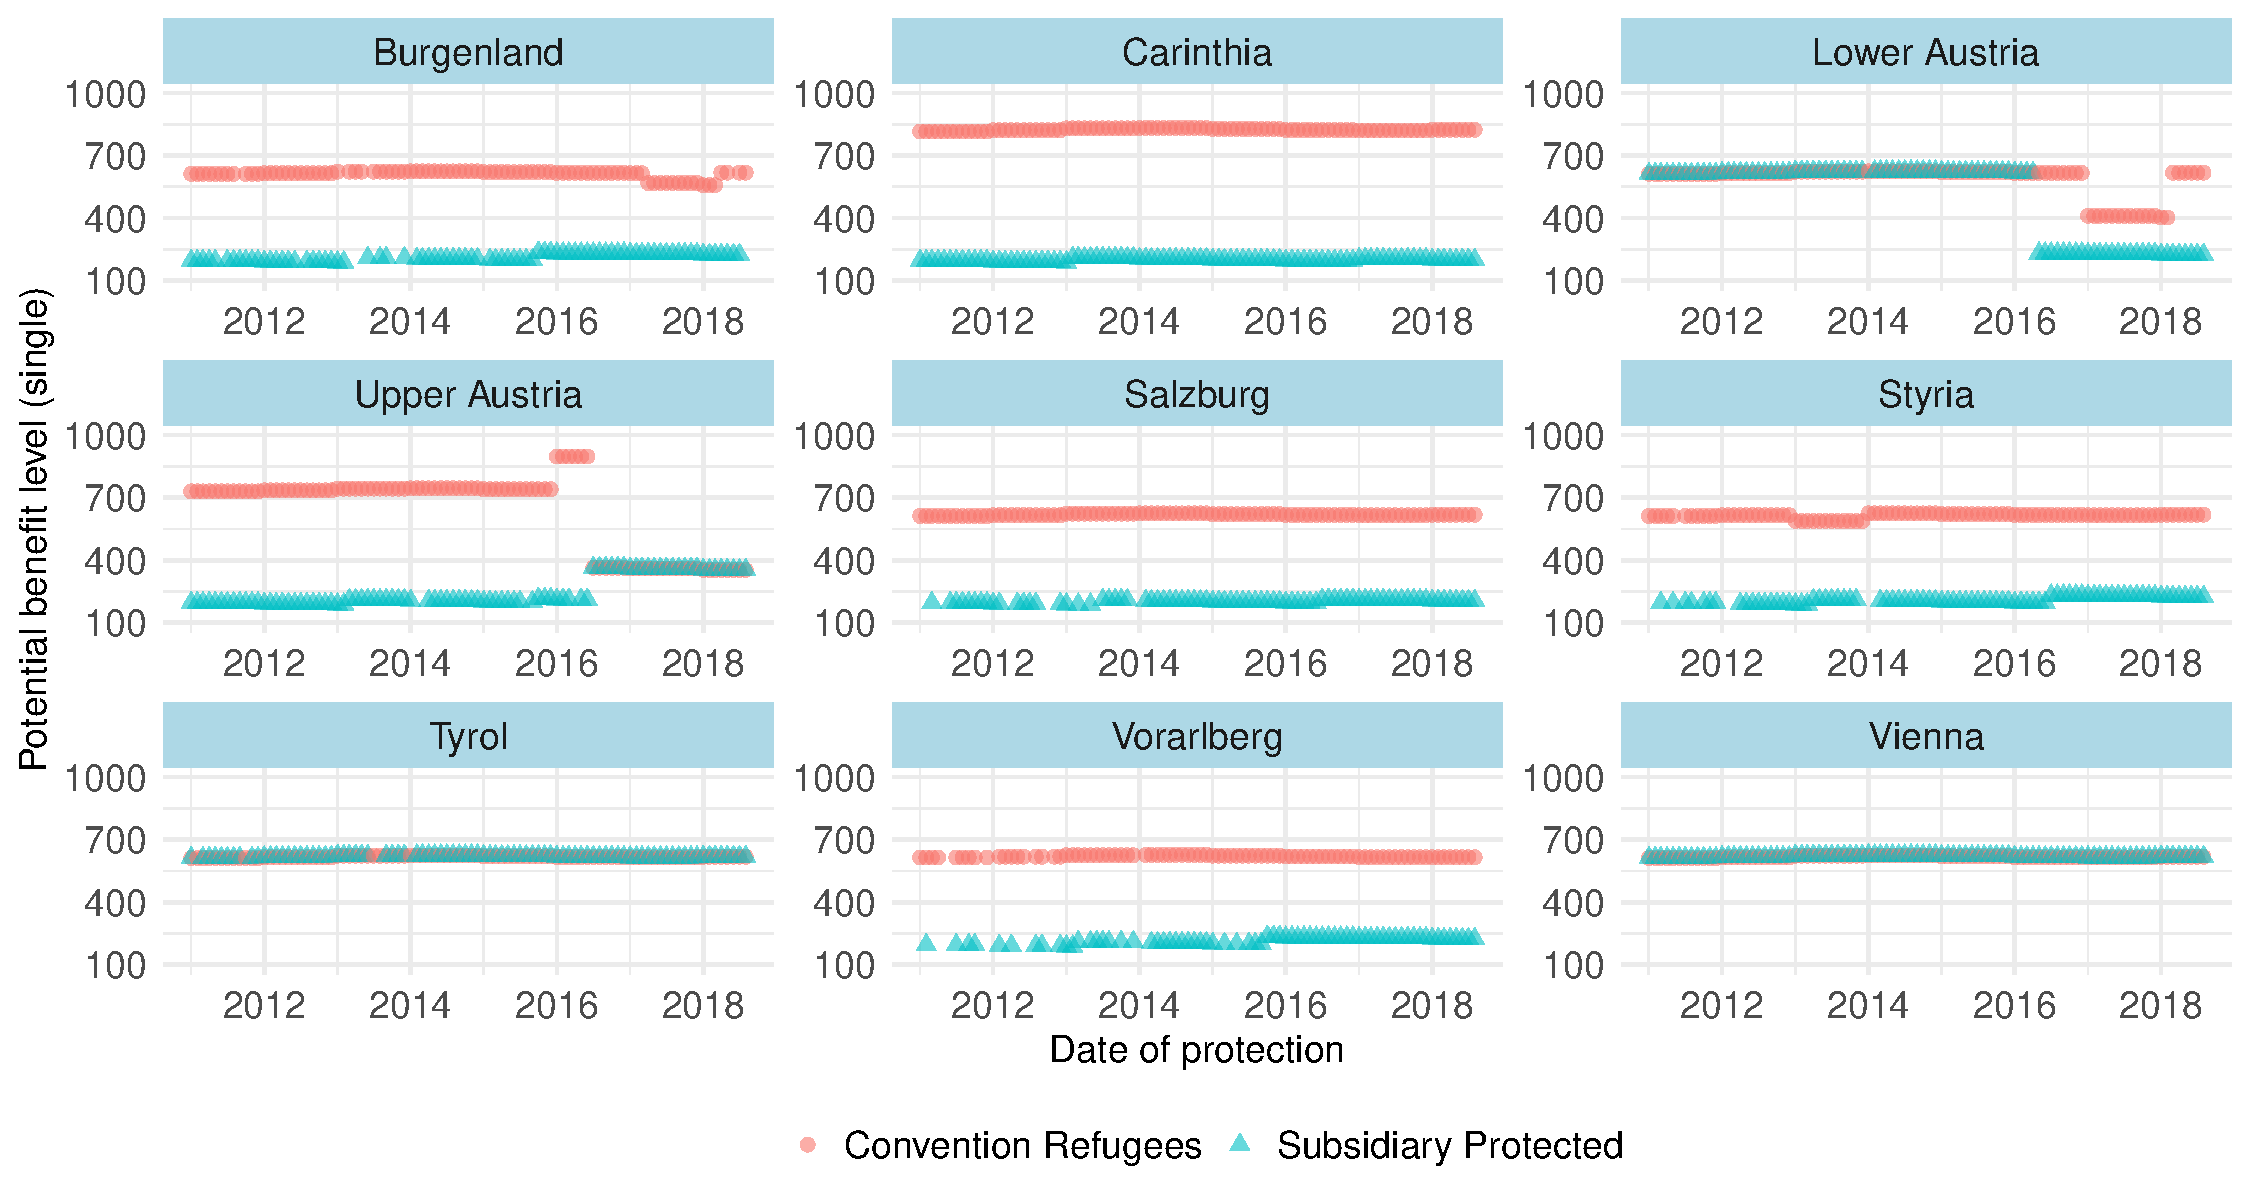
\includegraphics[scale=0.4]{figures/fig_ipbl.pdf}
    \end{center}
    \vspace{-0.7cm}
    \justify 
 		{\footnotesize 
 			\textit{Notes:}
    %\fignote{Notes: 
    The figure shows the amount of monthly benefits in euros (excluding housing benefits) for singles by federal state and type of protection.}
\end{figure}


\subsection*{Local economic conditions}

In addition to cross-state differences in benefit generosity, we exploit variation in the initial vacancy-to-unemployment ratio ($IVUR$) across districts over time.
Figure~\ref{fig:ivurmap} shows the average $IVUR$ during our period of analysis (2011--2018), providing a snapshot of the regional variation used in our analysis.

The graph shows that Vienna and districts in the eastern and southern states of the country display low average labor demand during this period.
 
These patterns are consistent with other labor market statistics at the state-level. For instance, Vienna exhibited the highest unemployment rate (8.4\%) in 2022 in Austria \citep{oecd_economy_aut}.

% \begin{figure}
%     \caption{Mean Vacancy-to-Unemployment Ratio by District}
%     \label{fig:ivurmap}
%     \begin{center}
%     \vspace{-0.5 cm}
%     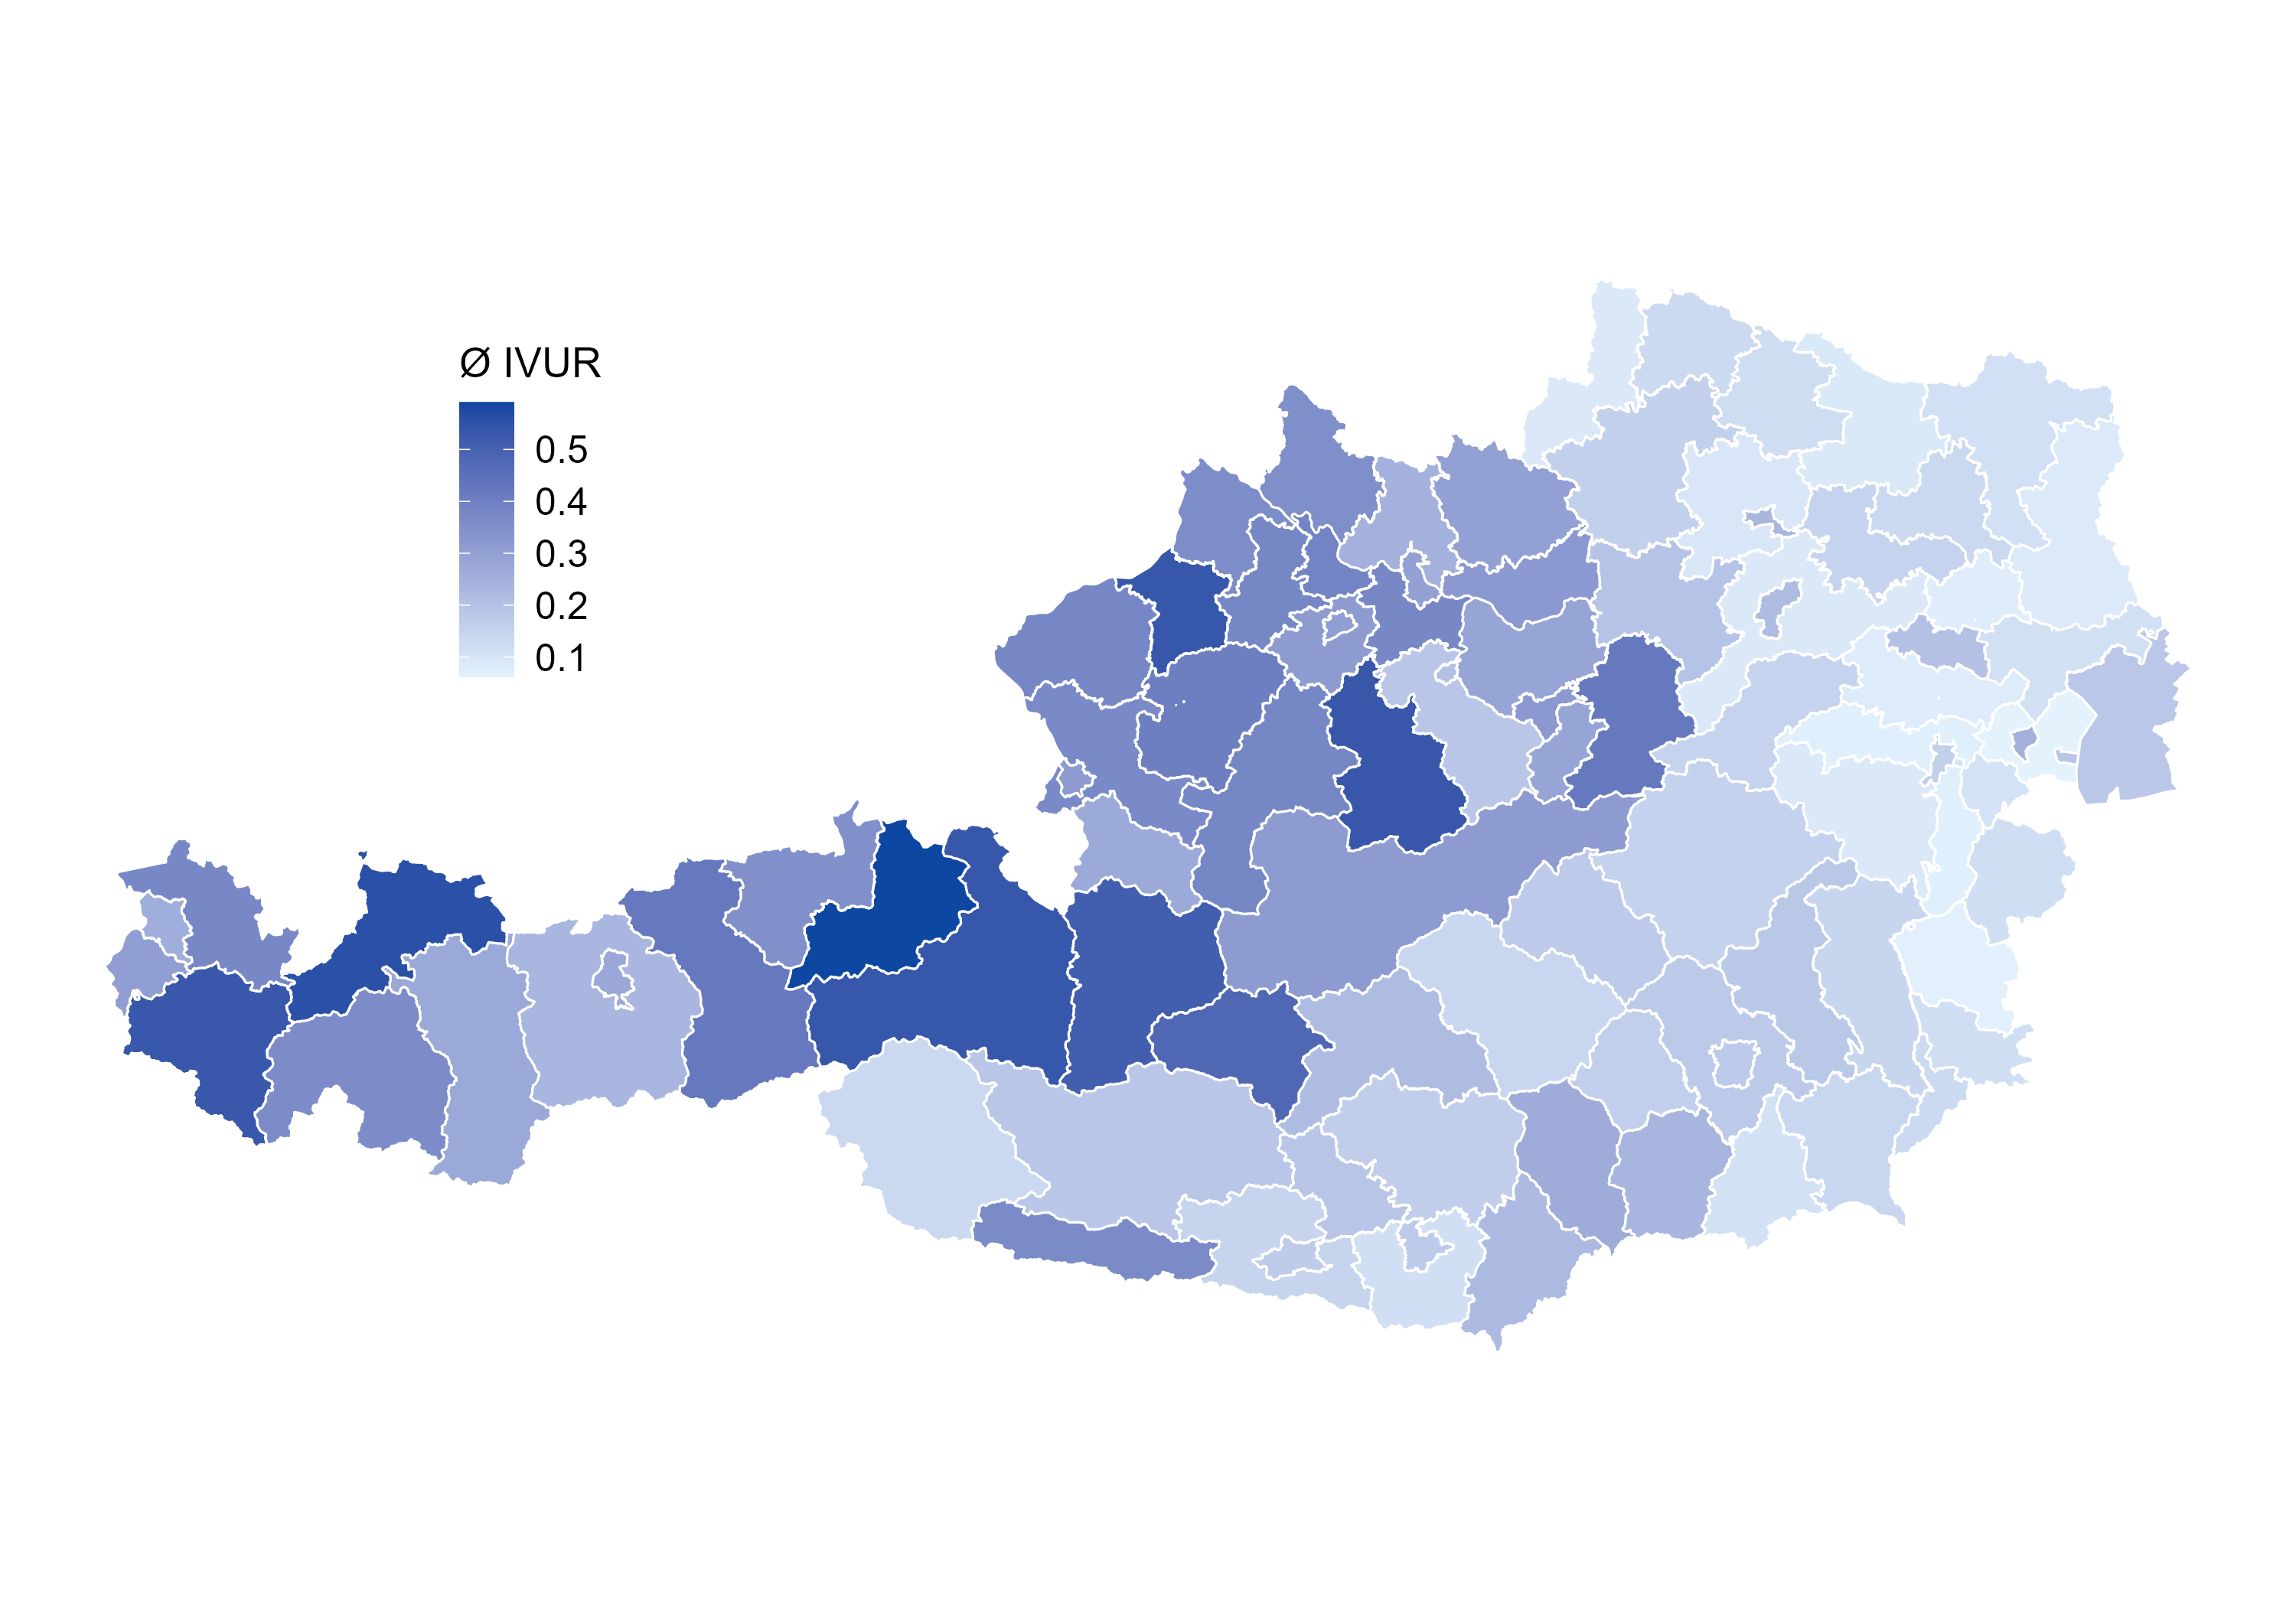
\includegraphics[scale=0.60]{figures/ivur_by_district_map.png}
%     \end{center}
%     \fignote{\footnotesize \textit{Notes:} 
% The map shows the mean vacancy-to-unemployment ratio ($IVUR$) by district, averaged across the period 2011–2018. District borders correspond to the NUTS 3 regional classification. Vienna is displayed as a single district.}
%     \vspace{-0.5 cm}
% \end{figure}

\begin{figure}
    \caption{Mean Vacancy-to-Unemployment Ratio by District}
    \label{fig:ivurmap}
    \begin{center}
    \vspace{-0.5 cm}
     \begin{tikzpicture}
    \node[anchor=south west,inner sep=0] (image) at (0,0) {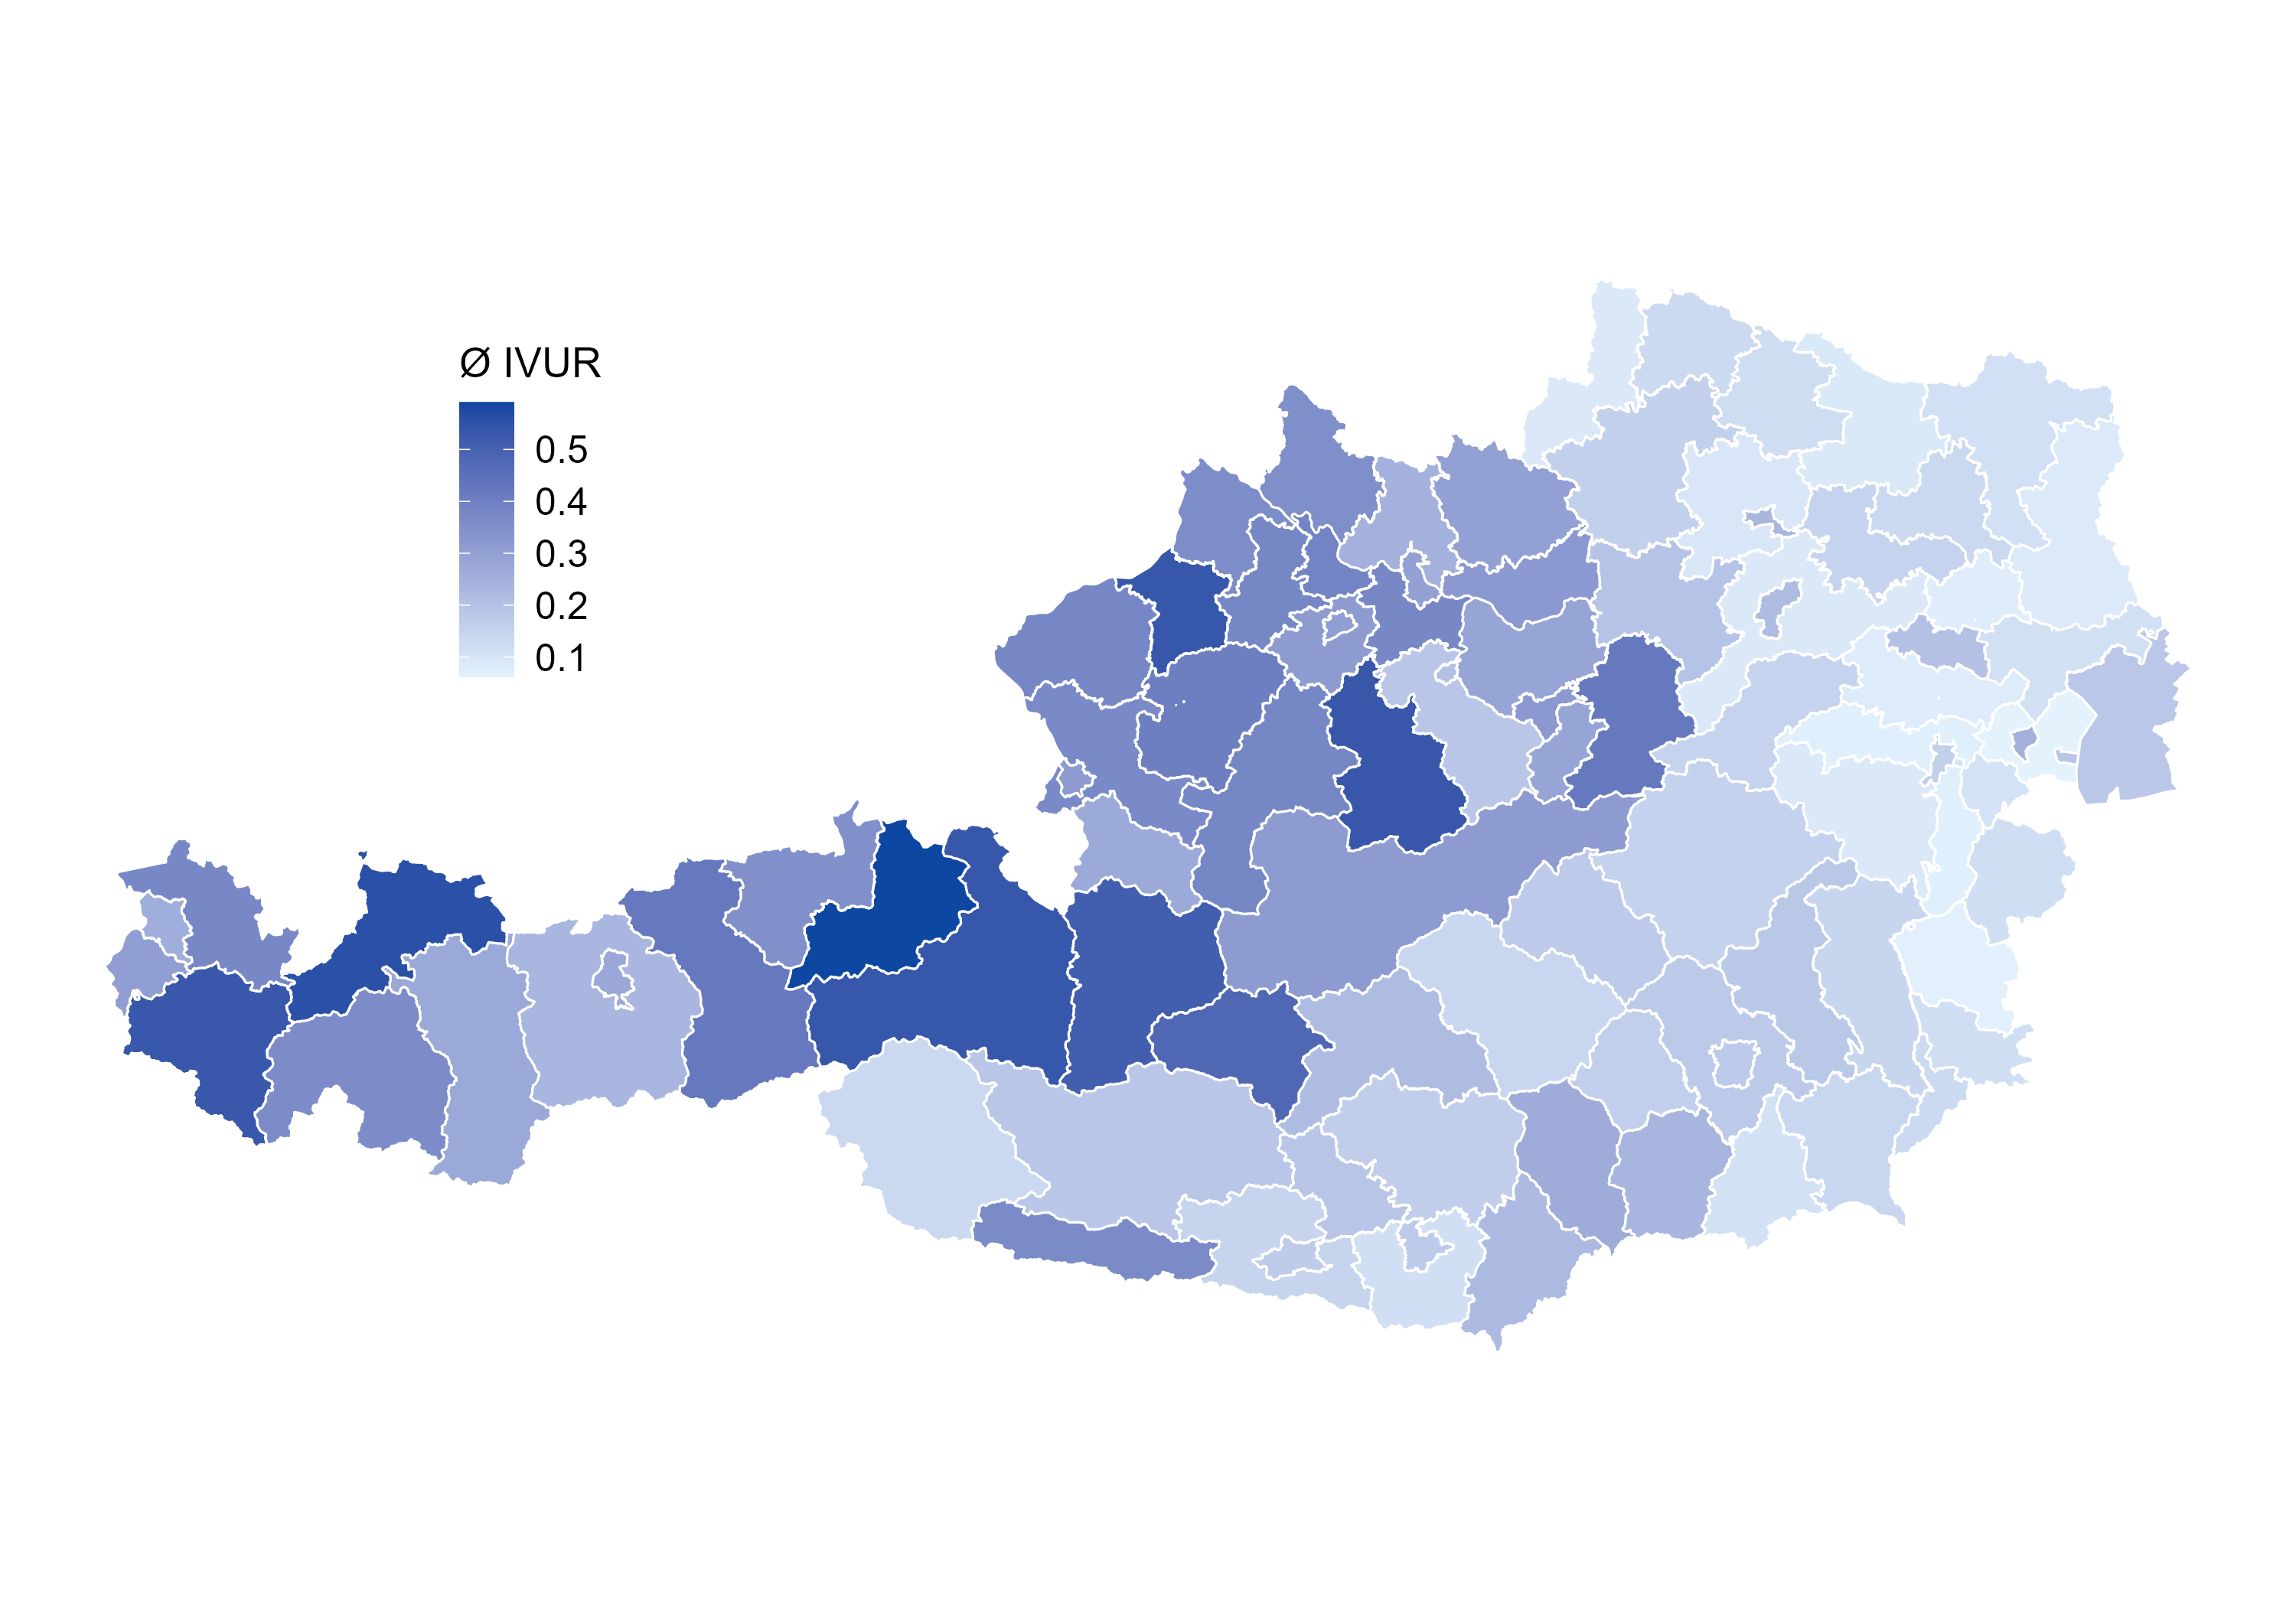
\includegraphics[width=\linewidth]{figures/ivur_by_district_map.png}};
    \begin{scope}[x={(image.south east)},y={(image.north west)}]
      % Arrow pointing to a location (x, y) in relative coordinates (0 to 1)
      \draw[<-, red, thick] (0.87, 0.63) -- (0.92, 0.68) node[above] {Vienna};
    \end{scope}
  \end{tikzpicture}
    \end{center}
    \fignote{\footnotesize \textit{Notes:} 
The map shows the mean vacancy-to-unemployment ratio ($IVUR$) by district, averaged across the period 2011–2018. District borders correspond to the NUTS 3 regional classification. Vienna is displayed as a single district.}
    \vspace{-0.5 cm}
\end{figure}

%\textbf{ADD SOME STATISTICS ON INFLOWS; COMPOSITION BY GENDER/FAMILY STATUS}


